\documentclass[10pt,a4paper]{article}
\usepackage[utf8]{inputenc}
\usepackage[T1]{fontenc}
\usepackage{amsmath}
\usepackage{amssymb}
\usepackage{graphicx}
\usepackage[english,russian]{babel} 
\usepackage{fontspec} 
\setmainfont{Times New Roman}
\title{Отчет по лабораторной работе №1}
\author{Ивлев А.Е Б19-511}
\usepackage{graphicx}
\graphicspath{{./Graphics/}}
\DeclareGraphicsExtensions{.pdf,.png,.jpg,.eps}
\begin{document}
	\maketitle
	
	\begin{figure}[h]
		\centering
		{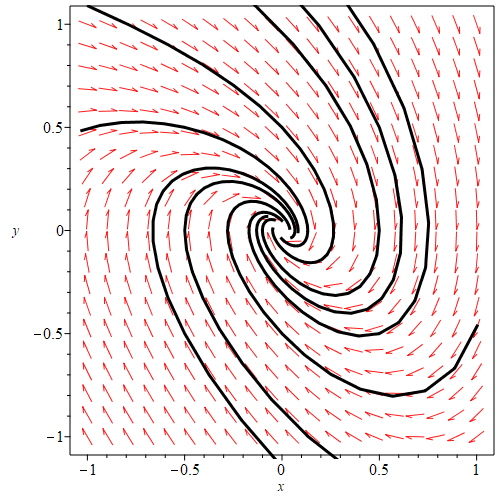
\includegraphics[scale=0.3]{phase_portrait, mu=1, alpha=1}}
		{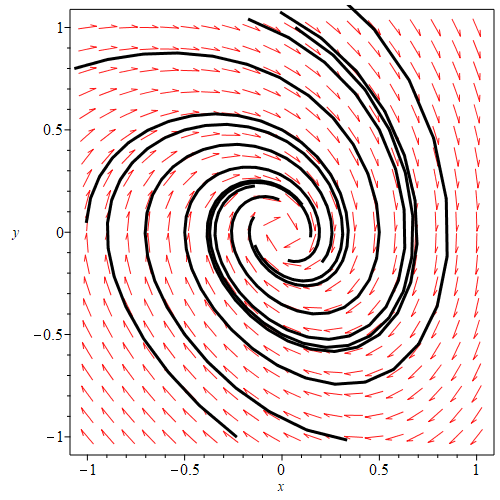
\includegraphics[scale=0.3]{phase_portrait, mu=1, alpha=0.5}}
		\caption{Фазовые портреты при $\mu = 1$, $\alpha = 1$; $\mu = 1$, $\alpha = 0.5$}
		\label{image/1}
	\end{figure}

	Исходная динамическая система:
	
	\begin{equation}
		\label{math/1}
		\ddot{x} + \mu \dot{x} + \alpha (\exp(x) - 1) = 0.	
	\end{equation}
	
	Она же в каноническом виде:
	\begin{equation}
		\label{math/2}
		\begin{cases}
			\dot{x} = y, \\
			\dot{y} = -\mu y - \alpha (\exp(x) - 1).
		\end{cases}
	\end{equation}

	Приравнивая правые части уравнения к нулю, находим точки покоя:
	\begin{equation}
		\label{math/3}
		\begin{cases}
			\ y = 0, \\
			\ -\mu y - \alpha (\exp(x) - 1) = 0.
		\end{cases}
	\end{equation}
	
	Единственная точка покоя - точка $(0;0)$.
	
	Матрица Якоби системы (\ref{math/1}) в точке покоя:
	\begin{equation}
		\label{math/4}
		\begin{bmatrix}
			0& 1\\
			-\alpha& -\mu
		\end{bmatrix}
	\end{equation}
	
	Собственные значения матрицы Якоби:
	\begin{equation}
		\label{math/5}
		\lambda_{1,2} = \frac{-\mu \pm \sqrt{\mu^{2} - 4\alpha}}{2}.
	\end{equation}
	
	Подбирая различные значения параметров, можно получить самые разные поведения системы. Рассмотрим случай $\alpha = 1$, $\mu = 1$. В таком случае собственные значения (\ref{math/5}) становятся комплексными, при этом их действительная часть меньше нуля.
	\begin{equation}
		\label{math/6}
		\lambda_{1,2} = -\frac{1}{2} \pm i \frac{\sqrt{3}}{2}.
	\end{equation}
	
	Следовательно можно сделать вывод о том, что фазовый портрет вблизи точки покоя представляет собой устойчивый фокус. Эти выводы подтверждаются численным построением фазового портрета в системе Maple (Рис.\ref{image/1}).
	
	Подобное поведение можно получить и при других значениях параметров $\mu$ и $\alpha$. Условия на параметры можно получить из (\ref{math/5}). Нужно потребовать, чтобы выражение под корней было отрицательным, а действительная часть была меньше нуля, то есть:
	\begin{equation}
		\label{math/7}
		\begin{cases}
			\alpha > \mu^2/4,  \\
			\mu > 0.
		\end{cases}
	\end{equation}
	
	
\end{document}